\documentclass[10pt]{article}
% Verification report for Dr. Sodhi, Dr. Jahangiri and Dr. Jeong (separate from ../cfd_2026-10/cfd_summary.tex).
% Build: python3 make_figures.py && latexmk -pdf -interaction=nonstopmode -halt-on-error cfd_verification.tex
% Every result, estimate, count and cost is a macro from numbers.tex (written by make_figures.py, source in a
% comment on each line); a number with no data yet prints "pending". Case labels (alpha, lambda, Ks, t, maxCo,
% FS, set numbers) and dates are typed. 10 pt (the 28 Oct summary used 11 pt) keeps the draft to six pages.
% figB1_checks.pdf (B1 results against the existing values) is drawn for the revision after B1; not used here.
\newcommand{\ReportDate}{Draft, 15 November 2026}
% Preamble for the roughness technical report. Numbers are NOT typed here:
% they come from ../build/numbers.tex, generated by src/build_report.py.
\usepackage[T1]{fontenc}
\usepackage[utf8]{inputenc}
\usepackage{lmodern}
\usepackage[scaled=0.92]{helvet}
\usepackage[letterpaper,margin=1in,headheight=14pt]{geometry}
\usepackage{microtype}
\usepackage{amsmath}
\usepackage{graphicx}
\usepackage{booktabs,tabularx,array,makecell,longtable,threeparttable}
\usepackage[per-mode=symbol,detect-all]{siunitx}
\usepackage[table]{xcolor}
\usepackage[font=small,labelfont=bf,labelsep=period,justification=raggedright,singlelinecheck=false]{caption}
\usepackage{subcaption}
\usepackage{enumitem}
\usepackage{float}
\usepackage{placeins}
\usepackage{fancyhdr}
\usepackage[nobottomtitles*]{titlesec}
\renewcommand{\bottomtitlespace}{0.12\textheight}
\usepackage{textcomp}
\usepackage{tikz}
\usetikzlibrary{positioning,arrows.meta}
\usepackage[hidelinks]{hyperref}
\hypersetup{pdfauthor={Stephen Eacuello}}
\widowpenalty=10000 \clubpenalty=10000
\hyphenation{time-stamps}

\definecolor{ink}{HTML}{0B0B0B}
\definecolor{ink2}{HTML}{52514E}
\definecolor{rule}{HTML}{C9C8C2}
\definecolor{navy}{HTML}{002147}
\definecolor{note}{HTML}{F4F3EF}
\definecolor{gold}{HTML}{B8860B}

\sisetup{group-minimum-digits=5, round-mode=none}
\setlist{nosep, leftmargin=1.4em}
\setlength{\parskip}{0.45em}
\setlength{\parindent}{0pt}
\renewcommand{\arraystretch}{1.12}

\titleformat{\section}{\normalfont\sffamily\Large\bfseries\color{navy}}{\thesection}{0.6em}{}
\titleformat{\subsection}{\normalfont\sffamily\large\bfseries\color{navy}}{\thesubsection}{0.6em}{}
\titleformat{\subsubsection}{\normalfont\sffamily\normalsize\bfseries}{\thesubsubsection}{0.6em}{}
\titlespacing*{\section}{0pt}{1.2em}{0.5em}
\titlespacing*{\subsection}{0pt}{1.0em}{0.35em}

\pagestyle{fancy}
\fancyhf{}
\fancyhead[L]{\sffamily\footnotesize\color{ink2}Peak power of a small VAWT with textured blades}
\fancyhead[R]{\sffamily\footnotesize\color{ink2}\ReportDate}
\fancyfoot[C]{\sffamily\footnotesize\color{ink2}\thepage}
\renewcommand{\headrulewidth}{0.4pt}

% A shaded box for the bottom line.
\newsavebox{\keyboxbin}
\newenvironment{keybox}{\par\smallskip\noindent\begin{lrbox}{\keyboxbin}%
  \begin{minipage}{\dimexpr\linewidth-2\fboxsep-1.2pt\relax}}%
  {\end{minipage}\end{lrbox}\fcolorbox{rule}{note}{\usebox{\keyboxbin}}\par\smallskip}

\newcommand{\Ra}[1]{\ensuremath{\mathrm{Ra}\,#1}}
\newcommand{\pmax}{P_{\max}}
\newcommand{\figref}[1]{Fig.~\ref{#1}}
\newcommand{\tabref}[1]{Table~\ref{#1}}
\newcommand{\secref}[1]{Section~\ref{#1}}
\newcommand{\appref}[1]{Appendix~\ref{#1}}
% \input is not expandable, which breaks it between booktabs rules; @@input is.
\makeatletter\newcommand{\tabinput}[1]{\@@input #1 }\makeatother

% numbers.tex: generated by make_figures.py; do not edit.
% Every number the report quotes, with its source (file, row, column) after the %.
\providecommand{\pending}{\textit{pending}}
\providecommand{\localonly}{\textit{local}}
\newcommand{\nGciCdNinety}{7.6}% cfd/analysis/2026-10-13/out/section_grid.csv alpha 90 Cd_mean GCI_fine_pct
\newcommand{\nSpreadClNinety}{24}% cfd/analysis/2026-10-13/out/section_grid.csv alpha 90 Cl_mean spread_pct_of_fine
\newcommand{\nSpreadCdZero}{9.0}% cfd/analysis/2026-10-13/out/section_grid.csv alpha 0 Cd_mean spread_pct_of_fine
\newcommand{\nSpreadCdOneEighty}{11.5}% cfd/analysis/2026-10-13/out/section_grid.csv alpha 180 Cd_mean spread_pct_of_fine
\newcommand{\nTsDropSST}{17.5}% cfd/analysis/2026-10-15/out/section_timestep_changes.csv alpha 180 SST maxCo 1.25 vs 2.5, -dCd_pct
\newcommand{\nTsDropLM}{14.8}% cfd/analysis/2026-10-15/out/section_timestep_changes.csv alpha 180 LM maxCo 1.25 vs 2.5, -dCd_pct
\newcommand{\nZeroCdFive}{3.19}% cfd/analysis/2026-10-15/out/section_timestep.csv alpha 0 SST maxCo 5 Cd (high-drag)
\newcommand{\nZeroCdTwoFive}{1.75}% cfd/analysis/2026-10-15/out/section_timestep.csv alpha 0 SST maxCo 2.5 Cd (low-drag)
\newcommand{\nZeroCdLastTen}{1.82}% cfd/analysis/2026-10-15/out/section_timestep.csv alpha 0 SST maxCo 1.25 Cd_last10
\newcommand{\nSurfCases}{74}% cfd/analysis/2026-11-15/out/surface_summary.csv rows
\newcommand{\nSCpWfNinetyZero}{\textminus{}1.64}% cfd/analysis/2026-11-15/out/surface_summary.csv a090.0_U23.0_SST_wf_Ks0_Tu1.0_Co2.5n2 Cp_min_B_1mm
\newcommand{\nSSepWfNinetyZero}{1.02}% cfd/analysis/2026-11-15/out/surface_summary.csv a090.0_U23.0_SST_wf_Ks0_Tu1.0_Co2.5n2 sep_B_from_stag_over_c
\newcommand{\nSCdpWfNinetyZero}{0.200}% cfd/analysis/2026-11-15/out/surface_summary.csv a090.0_U23.0_SST_wf_Ks0_Tu1.0_Co2.5n2 Cd_p_convex
\newcommand{\nSCpWfNinetyFour}{\textminus{}1.19}% cfd/analysis/2026-11-15/out/surface_summary.csv a090.0_U23.0_SST_wf_Ks400_Tu1.0_Co2.5n2 Cp_min_B_1mm
\newcommand{\nSSepWfNinetyFour}{0.96}% cfd/analysis/2026-11-15/out/surface_summary.csv a090.0_U23.0_SST_wf_Ks400_Tu1.0_Co2.5n2 sep_B_from_stag_over_c
\newcommand{\nSCdpWfNinetyFour}{0.290}% cfd/analysis/2026-11-15/out/surface_summary.csv a090.0_U23.0_SST_wf_Ks400_Tu1.0_Co2.5n2 Cd_p_convex
\newcommand{\nSCpTexZeroTwoFive}{\textminus{}3.19}% cfd/analysis/2026-11-15/out/surface_summary.csv a180.0_U23.0_SST_tex0.000_s1_Tu1.0_Co2.5n2 Cp_min_B_1mm
\newcommand{\nSSepTexZeroTwoFive}{0.69}% cfd/analysis/2026-11-15/out/surface_summary.csv a180.0_U23.0_SST_tex0.000_s1_Tu1.0_Co2.5n2 sep_B_from_stag_over_c
\newcommand{\nSCdpTexZeroTwoFive}{0.088}% cfd/analysis/2026-11-15/out/surface_summary.csv a180.0_U23.0_SST_tex0.000_s1_Tu1.0_Co2.5n2 Cd_p_convex
\newcommand{\nSCpTexTwoTwoFive}{\textminus{}1.81}% cfd/analysis/2026-11-15/out/surface_summary.csv a180.0_U23.0_SST_tex0.200_s1_Tu1.0_Co2.5n2 Cp_min_B_1mm
\newcommand{\nSSepTexTwoTwoFive}{0.55}% cfd/analysis/2026-11-15/out/surface_summary.csv a180.0_U23.0_SST_tex0.200_s1_Tu1.0_Co2.5n2 sep_B_from_stag_over_c
\newcommand{\nSCdpTexTwoTwoFive}{0.279}% cfd/analysis/2026-11-15/out/surface_summary.csv a180.0_U23.0_SST_tex0.200_s1_Tu1.0_Co2.5n2 Cd_p_convex
\newcommand{\nSCpTexZeroFive}{\textminus{}1.43}% cfd/analysis/2026-11-15/out/surface_summary.csv a180.0_U23.0_SST_tex0.000_s1_Tu1.0_N80A50 Cp_min_B_1mm
\newcommand{\nSSepTexZeroFive}{0.50}% cfd/analysis/2026-11-15/out/surface_summary.csv a180.0_U23.0_SST_tex0.000_s1_Tu1.0_N80A50 sep_B_from_stag_over_c
\newcommand{\nSCdpTexZeroFive}{0.287}% cfd/analysis/2026-11-15/out/surface_summary.csv a180.0_U23.0_SST_tex0.000_s1_Tu1.0_N80A50 Cd_p_convex
\newcommand{\nSCpTexTwoFive}{\textminus{}1.39}% cfd/analysis/2026-11-15/out/surface_summary.csv a180.0_U23.0_SST_tex0.200_s1_Tu1.0_N80A50 Cp_min_B_1mm
\newcommand{\nSSepTexTwoFive}{0.50}% cfd/analysis/2026-11-15/out/surface_summary.csv a180.0_U23.0_SST_tex0.200_s1_Tu1.0_N80A50 sep_B_from_stag_over_c
\newcommand{\nSCdpTexTwoFive}{0.317}% cfd/analysis/2026-11-15/out/surface_summary.csv a180.0_U23.0_SST_tex0.200_s1_Tu1.0_N80A50 Cd_p_convex
\newcommand{\nSCpMedTwoFive}{\textminus{}2.90}% cfd/analysis/2026-11-15/out/surface_summary.csv a180.0_U23.0_SST_medium_Tu1.0_Co2.5n2 Cp_min_B_1mm
\newcommand{\nSSepMedTwoFive}{0.62}% cfd/analysis/2026-11-15/out/surface_summary.csv a180.0_U23.0_SST_medium_Tu1.0_Co2.5n2 sep_B_from_stag_over_c
\newcommand{\nSCdpMedTwoFive}{0.081}% cfd/analysis/2026-11-15/out/surface_summary.csv a180.0_U23.0_SST_medium_Tu1.0_Co2.5n2 Cd_p_convex
\newcommand{\nSCpMedOneTwoFive}{\textminus{}1.76}% cfd/analysis/2026-11-15/out/surface_summary.csv a180.0_U23.0_SST_medium_Tu1.0_Co1.25n2 Cp_min_B_1mm
\newcommand{\nSSepMedOneTwoFive}{0.52}% cfd/analysis/2026-11-15/out/surface_summary.csv a180.0_U23.0_SST_medium_Tu1.0_Co1.25n2 sep_B_from_stag_over_c
\newcommand{\nSCdpMedOneTwoFive}{0.244}% cfd/analysis/2026-11-15/out/surface_summary.csv a180.0_U23.0_SST_medium_Tu1.0_Co1.25n2 Cd_p_convex
\newcommand{\nSSepShiftNinety}{0.07}% cfd/analysis/2026-11-15/out/surface_summary.csv sep_B_from_stag_over_c, a090.0_U23.0_SST_wf_Ks0_Tu1.0_Co2.5n2 minus a090.0_U23.0_SST_wf_Ks400_Tu1.0_Co2.5n2 (chords)
\newcommand{\nSSepShiftTex}{0.14}% cfd/analysis/2026-11-15/out/surface_summary.csv sep_B_from_stag_over_c, a180.0_U23.0_SST_tex0.000_s1_Tu1.0_Co2.5n2 minus a180.0_U23.0_SST_tex0.200_s1_Tu1.0_Co2.5n2 (chords)
\newcommand{\nSSepShiftMed}{0.10}% cfd/analysis/2026-11-15/out/surface_summary.csv sep_B_from_stag_over_c, a180.0_U23.0_SST_medium_Tu1.0_Co2.5n2 minus a180.0_U23.0_SST_medium_Tu1.0_Co1.25n2 (chords)
\newcommand{\nPressShareMin}{95.3}% section_polars.csv min Cd_pressure_mean/Cd_mean over the 102 runs with corrupted False in cfd/analysis/2026-10-15/out/section_case_quality.csv
\newcommand{\nPressViscMax}{4.7}% 100 - nPressShareMin: largest viscous share of Cd over the healthy section runs
\newcommand{\nHealthyRuns}{102}% cfd/analysis/2026-10-15/out/section_case_quality.csv corrupted False
\newcommand{\nBoneJobs}{25}% 23 active lines of cfd/stage2/queues/S2f_verify.txt, cfd/section2d/queues/priority7_verify.txt, cfd/rotor2d/queues/priorityF_verify.txt + 2 restarts named in priority7_verify.txt
\newcommand{\nBoneQueueJobs}{23}% active lines of cfd/stage2/queues/S2f_verify.txt, cfd/section2d/queues/priority7_verify.txt, cfd/rotor2d/queues/priorityF_verify.txt
\newcommand{\nBoneCoreLo}{7{,}500}% sum of the queue-header estimates (stated_values.csv b1_*) + the restarts' case.json estimate_steps x estimate_s_per_step x ranks
\newcommand{\nBoneCoreHi}{14{,}400}% as nBoneCoreLo
\newcommand{\nRestartCoreH}{304}% cfd/section2d/runs/{_cont,_hyst}*/case.json restart estimates (local)
\newcommand{\nBoneLongestDays}{3.6}% stated_values.csv b1_longest_days: cfd/stage2/queues/S2f_verify.txt (header, Cost)
\newcommand{\nRunsSec}{125}% cfd/section2d/results/section_polars.csv rows (October)
\newcommand{\nRunsWf}{37}% cfd/stage2/results/stage2_polars.csv rows, wall wf
\newcommand{\nRunsTex}{32}% cfd/stage2/results/stage2_polars.csv rows, wall tex
\newcommand{\nRunsRotor}{69}% cfd/rotor2d/results/rotor_cp.csv + rotor_static.csv rows
\newcommand{\nRunsAll}{263}% sum of the four
\newcommand{\nRunsSecSST}{35}% section_polars.csv rows, model SST
\newcommand{\nRunsSecLM}{90}% section_polars.csv rows, model LM
\newcommand{\nRunsTexSST}{12}% stage2_polars.csv rows, wall tex, model SST
\newcommand{\nRunsTexLM}{20}% stage2_polars.csv rows, wall tex, model LM
\newcommand{\nRunsRotRot}{53}% cfd/rotor2d/results/rotor_cp.csv rows (rotating)
\newcommand{\nRunsRotStat}{16}% cfd/rotor2d/results/rotor_static.csv rows (static)
\newcommand{\nCellsRotLo}{33}% rotor_cp.csv n_cells, coarse mesh of assembly A (thousands)
\newcommand{\nCellsRotHi}{119}% rotor_cp.csv n_cells, fine mesh of assembly A (thousands)
\newcommand{\nCellsSecLo}{69}% section_polars.csv n_cells, coarse grid cases (thousands)
\newcommand{\nCellsSecHi}{256}% section_polars.csv n_cells, fine grid cases (thousands)
\newcommand{\nCellsWf}{103}% stage2_polars.csv n_cells, wf rows, median (thousands)
\newcommand{\nCellsTex}{217}% stage2_polars.csv n_cells, tex rows, median (thousands)
\newcommand{\nYplusWfLo}{17}% stage2_polars.csv yplus_blade_mean, wf rows, min
\newcommand{\nYplusWfHi}{49}% stage2_polars.csv yplus_blade_mean, wf rows, max
\newcommand{\nKsOverYpMax}{0.91}% stage2_polars.csv Ks_over_yP, wf rows, max
\newcommand{\nCdWfSmooth}{1.62}% cfd/analysis/2026-10-15/out/roughness_wf_effects.csv a180.0 Ks0 Co2.5n2 Cd (smooth reference of the rough-wall family)
\newcommand{\nKspSmoothLimit}{2.25}% stated_values.csv wf_ksplus_smooth: cfd/docs/ROUGHNESS_KS.md section 1; cfd/stage2/README.md section 3 (nutkRoughWallFunction, v2606 source read 8 Oct)
\newcommand{\nKspRoughLimit}{90}% stated_values.csv wf_ksplus_rough: cfd/docs/ROUGHNESS_KS.md section 1 (v2606 source read 8 Oct)
\newcommand{\nWfNinetyTwoFive}{45.4}% cfd/analysis/2026-10-15/out/roughness_wf_effects.csv a090.0 Ks400 Co2.5n2 dCd_pct
\newcommand{\nWfNinetyFive}{44.4}% cfd/analysis/2026-10-15/out/roughness_wf_effects.csv a090.0 Ks400 (maxCo 5) dCd_pct
\newcommand{\nWfOneEightyTwoFive}{5.5}% cfd/analysis/2026-10-15/out/roughness_wf_effects.csv a180.0 Ks400 Co2.5n2 dCd_pct
\newcommand{\nWfMaxMove}{1.0}% cfd/analysis/2026-10-15/out/roughness_wf_effects.csv max |dCd_pct(maxCo 2.5) - dCd_pct(maxCo 5)|, alpha 90 and 180, Ks 50-400
\newcommand{\nWfLevelMove}{1.2}% cfd/analysis/2026-10-15/out/roughness_wf_effects.csv Ks0 Cd, |Co2.5n2/maxCo 5 - 1|, larger of alpha 90 and 180
\newcommand{\nWfNinetyFifty}{+0.73}% cfd/analysis/2026-10-15/out/roughness_wf_effects.csv a090.0 Ks50 Co2.5n2 dCd_pct
\newcommand{\nWfNinetyHundred}{+4.8}% cfd/analysis/2026-10-15/out/roughness_wf_effects.csv a090.0 Ks100 Co2.5n2 dCd_pct
\newcommand{\nWfOneEightyFifty}{+0.19}% cfd/analysis/2026-10-15/out/roughness_wf_effects.csv a180.0 Ks50 Co2.5n2 dCd_pct
\newcommand{\nWfOneEightyHundred}{+0.75}% cfd/analysis/2026-10-15/out/roughness_wf_effects.csv a180.0 Ks100 Co2.5n2 dCd_pct
\newcommand{\nKspSecLo}{2}% cfd/analysis/2026-10-15/out/roughness_wf_effects.csv ksplus_mean (maxCo 2.5) interpolated in Ks at k = 38 um, min of alpha 90/180
\newcommand{\nKspSecHi}{7}% cfd/analysis/2026-10-15/out/roughness_wf_effects.csv ksplus_mean interpolated at k = 97 um, max of alpha 90/180
\newcommand{\nKspSecFourLo}{26}% cfd/analysis/2026-10-15/out/roughness_wf_effects.csv ksplus_mean Ks400 Co2.5n2, min of alpha 90/180
\newcommand{\nKspSecFourHi}{38}% cfd/analysis/2026-10-15/out/roughness_wf_effects.csv ksplus_mean Ks400 Co2.5n2, max of alpha 90/180
\newcommand{\nTexDropSmooth}{17.5}% cfd/analysis/2026-10-15/out/roughness_tex_timestep.csv 180 SST t 0, -d_same_window_pct (maxCo 5 to 2.5)
\newcommand{\nTexDropTex}{16.2}% cfd/analysis/2026-10-15/out/roughness_tex_timestep.csv 180 SST t 0.2, -d_same_window_pct
\newcommand{\nTexEffFive}{13.7}% cfd/analysis/2026-10-15/out/roughness_tex_effects.csv a180 SST t 0.2 N80A50 (maxCo 5, 30-80 c/U) dCd_pct
\newcommand{\nTexEffTwoFiveShort}{15.5}% cfd/analysis/2026-10-15/out/roughness_tex_effects.csv a180 SST t 0.2 Co2.5n2 dCd_pct_30_80
\newcommand{\nTexEffLong}{13.6}% cfd/analysis/2026-10-15/out/roughness_tex_effects.csv a180 SST t 0.2 Co2.5n2 (50-150 c/U) dCd_pct
\newcommand{\nWinShortLo}{30}% cfd/analysis/2026-10-15/out/roughness_tex_effects.csv window of the maxCo-5 runs
\newcommand{\nWinShortHi}{80}% as nWinShortLo
\newcommand{\nWinLongLo}{50}% cfd/analysis/2026-10-15/out/roughness_tex_effects.csv window of the maxCo-2.5 runs
\newcommand{\nWinLongHi}{150}% as nWinLongLo
\newcommand{\nTexCdSmooth}{0.903}% stage2_polars.csv a180.0_U23.0_SST_tex0.000_s1_Tu1.0_Co2.5n2 Cd_mean
\newcommand{\nMedCdTwoFive}{1.479}% section_polars.csv a180.0_U23.0_SST_medium_Tu1.0_Co2.5n2 Cd_mean
\newcommand{\nMedCdOneTwoFive}{1.220}% section_polars.csv a180.0_U23.0_SST_medium_Tu1.0_Co1.25n2 Cd_mean
\newcommand{\nTexGapPct}{39}% 1 - Cd_mean(stage2 tex0.000 Co2.5n2) / Cd_mean(section medium Co2.5n2), alpha 180
\newcommand{\nTexGapMatched}{9.2}% 1 - Cd_mean(stage2 tex0.000 N80A50, window 30-80) / Cd_mean(section medium Co1.25n2, 50-150), alpha 180
\newcommand{\nTexGapDt}{0.6}% |dt_mean_s(stage2 tex0.000 N80A50) / dt_mean_s(section medium Co1.25n2) - 1|
\newcommand{\nRaPlain}{12.7}% reports/roughness_2026-09/build/derived/surface_roughness.csv Plain Ra_lc025_um
\newcommand{\nTeqPlain}{0.032}% reports/roughness_2026-09/build/derived/surface_roughness.csv Plain Ra_lc025_um / ra_per_t / 1000 (mm)
\newcommand{\nScansPlain}{1}% reports/roughness_2026-09/build/derived/surface_roughness.csv Plain scans
\newcommand{\nLayerPlain}{0.2}% reports/roughness_2026-09/build/derived/surface_roughness.csv Plain layer_period_um / 1000 (mm)
\newcommand{\nRaFsFive}{9.4}% reports/roughness_2026-09/build/derived/surface_roughness.csv FS 0.05 Ra_lc025_um
\newcommand{\nTeqFsFive}{0.024}% reports/roughness_2026-09/build/derived/surface_roughness.csv FS 0.05 Ra_lc025_um / ra_per_t / 1000 (mm)
\newcommand{\nScansFsFive}{1}% reports/roughness_2026-09/build/derived/surface_roughness.csv FS 0.05 scans
\newcommand{\nLayerFsFive}{0.1}% reports/roughness_2026-09/build/derived/surface_roughness.csv FS 0.05 layer_period_um / 1000 (mm)
\newcommand{\nRaFsTen}{8.2}% reports/roughness_2026-09/build/derived/surface_roughness.csv FS 0.10 Ra_lc025_um
\newcommand{\nTeqFsTen}{0.021}% reports/roughness_2026-09/build/derived/surface_roughness.csv FS 0.10 Ra_lc025_um / ra_per_t / 1000 (mm)
\newcommand{\nScansFsTen}{1}% reports/roughness_2026-09/build/derived/surface_roughness.csv FS 0.10 scans
\newcommand{\nLayerFsTen}{0.1}% reports/roughness_2026-09/build/derived/surface_roughness.csv FS 0.10 layer_period_um / 1000 (mm)
\newcommand{\nRaFsTwenty}{10.3}% reports/roughness_2026-09/build/derived/surface_roughness.csv FS 0.20 Ra_lc025_um
\newcommand{\nTeqFsTwenty}{0.026}% reports/roughness_2026-09/build/derived/surface_roughness.csv FS 0.20 Ra_lc025_um / ra_per_t / 1000 (mm)
\newcommand{\nScansFsTwenty}{2}% reports/roughness_2026-09/build/derived/surface_roughness.csv FS 0.20 scans
\newcommand{\nTeqLo}{0.021}% min of nTeq*
\newcommand{\nTeqHi}{0.032}% max of nTeq*
\newcommand{\nKsEqLo}{43}% ks_per_t x Ra / ra_per_t, min over the four tested sets (um)
\newcommand{\nKsEqHi}{67}% as nKsEqLo, max
\newcommand{\nNomOverRaLo}{2}% ra_per_t x t / measured Ra (reports/roughness_2026-09/build/derived/surface_roughness.csv), min over FS 0.05-0.20
\newcommand{\nNomOverRaHi}{8}% as nNomOverRaLo, max
\newcommand{\nGainFsFive}{+1.8}% cfd/analysis/2026-10-15/out/roughness_measured.csv FS 0.05 change_pct
\newcommand{\nGainFsFiveLo}{\textminus{}0.6}% cfd/analysis/2026-10-15/out/roughness_measured.csv FS 0.05 tukey95_lo_pct
\newcommand{\nGainFsFiveHi}{+4.2}% cfd/analysis/2026-10-15/out/roughness_measured.csv FS 0.05 tukey95_hi_pct
\newcommand{\nGainFsTen}{+12.8}% cfd/analysis/2026-10-15/out/roughness_measured.csv FS 0.10 change_pct
\newcommand{\nGainFsTenLo}{+10.1}% cfd/analysis/2026-10-15/out/roughness_measured.csv FS 0.10 tukey95_lo_pct
\newcommand{\nGainFsTenHi}{+15.5}% cfd/analysis/2026-10-15/out/roughness_measured.csv FS 0.10 tukey95_hi_pct
\newcommand{\nGainFsTwenty}{+16.2}% cfd/analysis/2026-10-15/out/roughness_measured.csv FS 0.20 change_pct
\newcommand{\nGainFsTwentyLo}{+13.5}% cfd/analysis/2026-10-15/out/roughness_measured.csv FS 0.20 tukey95_lo_pct
\newcommand{\nGainFsTwentyHi}{+19.0}% cfd/analysis/2026-10-15/out/roughness_measured.csv FS 0.20 tukey95_hi_pct
\newcommand{\nKLow}{38}% stated_values.csv k_low_um: reports/roughness_2026-09/MEETING_2026-10-07_Jahangiri.md ('Our numbers'); cfd/docs/ROUGHNESS_KS.md section 2
\newcommand{\nKHighLo}{84}% stated_values.csv k_fs20_lo_um: as k_low_um
\newcommand{\nKHighHi}{97}% stated_values.csv k_fs20_hi_um: as k_low_um
\newcommand{\nKsPerT}{2.09}% stated_values.csv ks_per_t: cfd/docs/ROUGHNESS_KS.md section 3
\newcommand{\nRaPerT}{0.397}% stated_values.csv ra_per_t: cfd/docs/ROUGHNESS_KS.md section 3; cfd/stage2/README.md section 4
\newcommand{\nKsNomFsFive}{104}% stated_values.csv ks_nom_fs05_um: cfd/docs/ROUGHNESS_KS.md section 3 (nominal-texture row)
\newcommand{\nKsNomFsTen}{211}% stated_values.csv ks_nom_fs10_um: cfd/docs/ROUGHNESS_KS.md section 3 (nominal-texture row)
\newcommand{\nKsNomFsTwenty}{422}% stated_values.csv ks_nom_fs20_um: cfd/docs/ROUGHNESS_KS.md section 3 (nominal-texture row)
\newcommand{\nKsNomFsForty}{835}% stated_values.csv ks_nom_fs40_um: cfd/docs/ROUGHNESS_KS.md section 3 (planned FS 0.40 row)
\newcommand{\nTFsFive}{0.050}% stated_values.csv t_fs05_mm: cfd/docs/ROUGHNESS_KS.md section 2
\newcommand{\nTFsTen}{0.101}% stated_values.csv t_fs10_mm: cfd/docs/ROUGHNESS_KS.md section 2
\newcommand{\nTFsTwenty}{0.202}% stated_values.csv t_fs20_mm: cfd/docs/ROUGHNESS_KS.md section 2
\newcommand{\nTFsQuarter}{0.025}% stated_values.csv t_fs025_mm: reports/roughness_2026-09/inputs/print_lab_20261012/README.md
\newcommand{\nTFsForty}{0.40}% stated_values.csv t_fs40_mm: reports/roughness_2026-09/outgoing/2026-10-22_print_request_cam.md (7 Oct follow-up)
\newcommand{\nTFsEighty}{0.805}% stated_values.csv t_fs80_mm: reports/roughness_2026-09/inputs/print_lab_20261012/README.md
\newcommand{\nLayerFsEighty}{0.12}% stated_values.csv layer_fs80_mm: reports/roughness_2026-09/inputs/print_lab_20261012/README.md
\newcommand{\nLayerSlicer}{0.1}% stated_values.csv layer_slicer_mm: reports/roughness_2026-09/inputs/print_lab_20261012/README.md (turbine_p2mm.3mf, 0.10mm Standard)
\newcommand{\nLayerLimit}{0.14}% stated_values.csv layer_limit_mm: reports/roughness_2026-09/inputs/print_lab_20261012/README.md (Points to confirm)
\newcommand{\nNozzleSmall}{0.2}% stated_values.csv nozzle_tested_mm: reports/roughness_2026-09/inputs/print_lab_20261012/README.md (Print Lab reply of 12 Oct)
\newcommand{\nNozzleLarge}{0.4}% stated_values.csv nozzle_large_mm: reports/roughness_2026-09/inputs/print_lab_20261012/README.md (turbine_320.3mf); November round set 1
\newcommand{\nSlicerMax}{1}% stated_values.csv slicer_max_fs_mm: November print round, sets 1-3 approved 9 Nov 2026 (not in the repo)
\newcommand{\nKsNomFsQuarter}{52}% ks_per_t x t_fs025_mm (um)
\newcommand{\nRotEffTen}{+0.0051}% cfd/analysis/2026-10-15/out/rotor_roughness.csv 0.1 Ks400-Ks0 dCQ
\newcommand{\nRotEffTenU}{0.0028}% cfd/analysis/2026-10-15/out/rotor_roughness.csv 0.1 Ks400-Ks0 two_u
\newcommand{\nRotEffTwelve}{+0.0058}% cfd/analysis/2026-10-15/out/rotor_roughness.csv 0.12 Ks400-Ks0 dCQ
\newcommand{\nRotEffTwelveU}{0.0028}% cfd/analysis/2026-10-15/out/rotor_roughness.csv 0.12 Ks400-Ks0 two_u
\newcommand{\nRotHunTen}{+0.0014}% cfd/analysis/2026-10-15/out/rotor_roughness.csv 0.1 Ks100-Ks0 dCQ
\newcommand{\nRotHunTenU}{0.0027}% cfd/analysis/2026-10-15/out/rotor_roughness.csv 0.1 Ks100-Ks0 two_u
\newcommand{\nRotHunTwelve}{\textminus{}0.0029}% cfd/analysis/2026-10-15/out/rotor_roughness.csv 0.12 Ks100-Ks0 dCQ
\newcommand{\nRotHunTwelveU}{0.0032}% cfd/analysis/2026-10-15/out/rotor_roughness.csv 0.12 Ks100-Ks0 two_u
\newcommand{\nRotEffTenPct}{27}% cfd/analysis/2026-10-15/out/rotor_roughness.csv 0.1 Ks400-Ks0 rel_change_pct
\newcommand{\nRotEffTwelvePct}{38}% cfd/analysis/2026-10-15/out/rotor_roughness.csv 0.12 Ks400-Ks0 rel_change_pct
\newcommand{\nRotTwoULo}{0.0027}% cfd/analysis/2026-10-15/out/rotor_roughness.csv two_u, Ks 100/400 - Ks 0 pairs, min
\newcommand{\nRotTwoUHi}{0.0032}% cfd/analysis/2026-10-15/out/rotor_roughness.csv two_u, Ks 100/400 - Ks 0 pairs, max
\newcommand{\nAdvHun}{+0.00112}% cfd/analysis/2026-10-15/out/rotor_roughness_sectors.csv 0.1 Ks100-Ks0 advancing d
\newcommand{\nAdvHunU}{0.00039}% cfd/analysis/2026-10-15/out/rotor_roughness_sectors.csv 0.1 Ks100-Ks0 advancing two_u
\newcommand{\nSecAdv}{+0.0092}% cfd/analysis/2026-10-15/out/rotor_roughness_sectors.csv 0.1 Ks400-Ks0 adv d
\newcommand{\nSecAdvU}{0.0006}% cfd/analysis/2026-10-15/out/rotor_roughness_sectors.csv 0.1 Ks400-Ks0 adv two_u
\newcommand{\nSecRet}{\textminus{}0.0048}% cfd/analysis/2026-10-15/out/rotor_roughness_sectors.csv 0.1 Ks400-Ks0 ret d
\newcommand{\nSecRetU}{0.0022}% cfd/analysis/2026-10-15/out/rotor_roughness_sectors.csv 0.1 Ks400-Ks0 ret two_u
\newcommand{\nSecDown}{+0.0032}% cfd/analysis/2026-10-15/out/rotor_roughness_sectors.csv 0.1 Ks400-Ks0 down d
\newcommand{\nSecDownU}{0.0011}% cfd/analysis/2026-10-15/out/rotor_roughness_sectors.csv 0.1 Ks400-Ks0 down two_u
\newcommand{\nSecUp}{\textminus{}0.0015}% cfd/analysis/2026-10-15/out/rotor_roughness_sectors.csv 0.1 Ks400-Ks0 up d
\newcommand{\nSecUpU}{0.0006}% cfd/analysis/2026-10-15/out/rotor_roughness_sectors.csv 0.1 Ks400-Ks0 up two_u
\newcommand{\nRotMeshFC}{+0.0116}% cfd/analysis/2026-10-15/out/rotor_numbers.json grid.differences.0.10.fine_minus_coarse
\newcommand{\nRotMeshFCU}{0.0110}% cfd/analysis/2026-10-15/out/rotor_numbers.json grid.differences.0.10.two_u_diff
\newcommand{\nRotMeshOverEff}{2.3}% nRotMeshFC / nRotEffTen
\newcommand{\nRotNrevGrid}{3}% cfd/analysis/2026-10-15/out/rotor_numbers.json grid.rows fine 0.1 n_avg_rev
\newcommand{\nRotTs}{\textminus{}0.0067}% cfd/analysis/2026-10-15/out/rotor_numbers.json time_step_check CCW dCQ (lambda 0.15, maxCo 4 to 2)
\newcommand{\nRotTsU}{0.0110}% cfd/analysis/2026-10-15/out/rotor_numbers.json time_step_check CCW 2 |dCQ / dCQ_over_u_diff|
\newcommand{\nKspRotLo}{3}% cfd/analysis/2026-10-15/out/rotor_numbers.json roughness.runs.*_Ks100/400.ksplus_mean interpolated in Ks at 38 um (min over lambda)
\newcommand{\nKspRotHi}{7}% as nKspRotLo, at 97 um (max over lambda)
\newcommand{\nKspRotFour}{33}% cfd/analysis/2026-10-15/out/rotor_numbers.json roughness.runs.0.10_Ks400.ksplus_mean
\newcommand{\nKsOverYpRot}{0.92}% cfd/analysis/2026-10-15/out/rotor_numbers.json roughness.runs.0.10_Ks400.Ks_over_yP
\newcommand{\nTrendLo}{0.0005}% cfd/analysis/2026-10-15/out/rotor_numbers.json roughness.ks_trend.0.10.slope_per_100um x 38/100
\newcommand{\nTrendHi}{0.0012}% cfd/analysis/2026-10-15/out/rotor_numbers.json roughness.ks_trend.0.10.slope_per_100um x 97/100
\newcommand{\nRevNeeded}{250}% 8 sigma^2 / d^2 with sigma = cfd/analysis/2026-10-15/out/rotor_numbers.json noise_model.sigma_long_runs_rms, d = nTrendHi (rounded to 10)
\newcommand{\nRevNow}{45}% cfd/rotor2d/results/rotor_cp.csv n_avg_rev of the lambda-0.10 Ks pair
\newcommand{\nCoreHPerRev}{3.7}% cfd/analysis/2026-10-15/out/rotor_numbers.json cost_long_runs wall_h x inputs.jobs_new ntasks / rotor_cp.csv n_rev_done, mean of 8 runs
\newcommand{\nPfRuns}{8}% cfd/analysis/2026-11-15/out/rotor_phase_force_sectors.csv distinct runs
\newcommand{\nPfAdvCD}{+0.077}% cfd/analysis/2026-11-15/out/rotor_phase_force_sectors.csv lambda 0.1 difference Ks400-Ks0 advancing CD
\newcommand{\nPfAdvCDU}{0.004}% cfd/analysis/2026-11-15/out/rotor_phase_force_sectors.csv lambda 0.1 difference Ks400-Ks0 advancing CD_2u
\newcommand{\nPfAdvCDPct}{18}% cfd/analysis/2026-11-15/out/rotor_phase_force_sectors.csv lambda 0.1 advancing CD difference / run Ks0 CD
\newcommand{\nPfAdvCL}{+0.20}% cfd/analysis/2026-11-15/out/rotor_phase_force_sectors.csv lambda 0.1 difference Ks400-Ks0 advancing CL
\newcommand{\nPfAdvCLU}{0.01}% cfd/analysis/2026-11-15/out/rotor_phase_force_sectors.csv lambda 0.1 difference Ks400-Ks0 advancing CL_2u
\newcommand{\nPfUpCD}{+0.067}% cfd/analysis/2026-11-15/out/rotor_phase_force_sectors.csv lambda 0.1 difference Ks400-Ks0 upwind CD
\newcommand{\nPfUpCDU}{0.004}% cfd/analysis/2026-11-15/out/rotor_phase_force_sectors.csv lambda 0.1 difference Ks400-Ks0 upwind CD_2u
\newcommand{\nPfUpCL}{+0.007}% cfd/analysis/2026-11-15/out/rotor_phase_force_sectors.csv lambda 0.1 difference Ks400-Ks0 upwind CL
\newcommand{\nPfUpCLU}{0.007}% cfd/analysis/2026-11-15/out/rotor_phase_force_sectors.csv lambda 0.1 difference Ks400-Ks0 upwind CL_2u
\newcommand{\nPfRetCD}{+0.043}% cfd/analysis/2026-11-15/out/rotor_phase_force_sectors.csv lambda 0.1 difference Ks400-Ks0 returning CD
\newcommand{\nPfRetCDU}{0.037}% cfd/analysis/2026-11-15/out/rotor_phase_force_sectors.csv lambda 0.1 difference Ks400-Ks0 returning CD_2u
\newcommand{\nPfBladeShare}{32}% cfd/analysis/2026-11-15/out/rotor_phase_force_check.csv blade-to-blade CD recomputed
\newcommand{\nPfBladeExpect}{5}% cfd/analysis/2026-11-15/out/rotor_phase_force_check.csv blade-to-blade CD reference
\newcommand{\nDwells}{2{,}754}% reports/roughness_2026-09/out/URI_VAWT_Texture_Data_2026-10-01_rev2/4_derived/rotor_speed_by_dwell.csv rows (load steps)
\newcommand{\nDwellsOk}{2{,}742}% reports/roughness_2026-09/out/URI_VAWT_Texture_Data_2026-10-01_rev2/4_derived/rotor_speed_by_dwell.csv speed_ok True
\newcommand{\nLamLightLo}{0.158}% reports/roughness_2026-09/out/URI_VAWT_Texture_Data_2026-10-01_rev2/4_derived/rotor_speed_by_dwell.csv fan_rpm_cmd 1100, per rotor and run: tip_speed_ratio at the lightest load, min
\newcommand{\nLamLightHi}{0.181}% reports/roughness_2026-09/out/URI_VAWT_Texture_Data_2026-10-01_rev2/4_derived/rotor_speed_by_dwell.csv fan_rpm_cmd 1100, per rotor and run: tip_speed_ratio at the lightest load, max
\newcommand{\nLamHeavyLo}{0.090}% reports/roughness_2026-09/out/URI_VAWT_Texture_Data_2026-10-01_rev2/4_derived/rotor_speed_by_dwell.csv fan_rpm_cmd 1100, per rotor and run: tip_speed_ratio at the heaviest load, min
\newcommand{\nLamHeavyHi}{0.105}% reports/roughness_2026-09/out/URI_VAWT_Texture_Data_2026-10-01_rev2/4_derived/rotor_speed_by_dwell.csv fan_rpm_cmd 1100, per rotor and run: tip_speed_ratio at the heaviest load, max
\newcommand{\nLamPmaxLo}{0.121}% reports/roughness_2026-09/out/URI_VAWT_Texture_Data_2026-10-01_rev2/4_derived/rotor_speed_by_dwell.csv fan_rpm_cmd 1100, per rotor and run: tip_speed_ratio at the largest cp_el, min
\newcommand{\nLamPmaxHi}{0.136}% reports/roughness_2026-09/out/URI_VAWT_Texture_Data_2026-10-01_rev2/4_derived/rotor_speed_by_dwell.csv fan_rpm_cmd 1100, per rotor and run: tip_speed_ratio at the largest cp_el, max
\newcommand{\nLocalJobs}{259}% cfd/*/runs/*/hpc_jobs.jsonl records started in Oct 2026 (local)
\newcommand{\nLocalCoreH}{15{,}145}% sum of wall_s x ntasks / 3600 over those records (local)
\newcommand{\nLocalCoreHSec}{7{,}012}% as nLocalCoreH, stage section2d
\newcommand{\nLocalCoreHStage}{5{,}969}% as nLocalCoreH, stage stage2
\newcommand{\nLocalCoreHRot}{2{,}164}% as nLocalCoreH, stage rotor2d
\newcommand{\nOctJobs}{281}% stated_values.csv oct_jobs: reports/cfd_2026-10/cfd_summary.tex, What we simulated
\newcommand{\nOctCoreH}{17{,}400}% stated_values.csv oct_core_h: reports/cfd_2026-10/cfd_summary.tex, What we simulated
\newcommand{\nUnityDays}{5}% stated_values.csv unity_max_days: cfd/hpc/README.md (How it works, Jobs)
\newcommand{\nBTwoLo}{2{,}900}% stated_values.csv b2_lo: approved plan of 15 Nov 2026, Step 4 (not in the repo)
\newcommand{\nBTwoHi}{7{,}600}% stated_values.csv b2_hi: approved plan of 15 Nov 2026, Step 4 (not in the repo)
\newcommand{\nTexRotRevLo}{100}% stated_values.csv texrotor_rev_lo: approved plan of 15 Nov 2026 (not in the repo)
\newcommand{\nTexRotRevHi}{1{,}600}% stated_values.csv texrotor_rev_hi: approved plan of 15 Nov 2026 (not in the repo)
\newcommand{\nTexRotPairLo}{3{,}100}% stated_values.csv texrotor_pair_lo: approved plan of 15 Nov 2026 (not in the repo)
\newcommand{\nTexRotPairHi}{49{,}000}% stated_values.csv texrotor_pair_hi: approved plan of 15 Nov 2026 (not in the repo)
\newcommand{\nLmRotLo}{1{,}150}% stated_values.csv lmrotor_lo: approved plan of 15 Nov 2026, Step 5 (not in the repo)
\newcommand{\nLmRotHi}{2{,}300}% stated_values.csv lmrotor_hi: approved plan of 15 Nov 2026, Step 5 (not in the repo)
\newcommand{\nStripLo}{6{,}700}% stated_values.csv strip_lo: approved plan of 15 Nov 2026 (not in the repo)
\newcommand{\nStripHi}{108{,}000}% stated_values.csv strip_hi: approved plan of 15 Nov 2026 (not in the repo)
\newcommand{\nBladeCellsLo}{1}% stated_values.csv blade3d_gcells_lo: approved plan of 15 Nov 2026 (not in the repo)
\newcommand{\nBladeCellsHi}{4}% stated_values.csv blade3d_gcells_hi: approved plan of 15 Nov 2026 (not in the repo)
\newcommand{\nBladeCoreLo}{0.8}% stated_values.csv blade3d_mcoreh_lo: approved plan of 15 Nov 2026 (not in the repo)
\newcommand{\nBladeCoreHi}{20}% stated_values.csv blade3d_mcoreh_hi: approved plan of 15 Nov 2026 (not in the repo)
\newcommand{\nTunnelLo}{28}% stated_values.csv tunnel_h_lo: approved plan of 15 Nov 2026 (not in the repo)
\newcommand{\nTunnelHi}{31}% stated_values.csv tunnel_h_hi: approved plan of 15 Nov 2026 (not in the repo)
\newcommand{\nAccLevel}{5}% stated_values.csv acc_level_pct: cfd/stage2/queues/S2f_verify.txt (header, Acceptance)
\newcommand{\nAccEff}{5}% stated_values.csv acc_effect_pts: cfd/stage2/queues/S2f_verify.txt (header, Acceptance)
\newcommand{\nAccCostLo}{1.4}% stated_values.csv acc_cost_lo: cfd/stage2/queues/S2f_verify.txt (header, Acceptance)
\newcommand{\nAccCostHi}{3.1}% stated_values.csv acc_cost_hi: cfd/stage2/queues/S2f_verify.txt (header, Acceptance)
\newcommand{\nAccRot}{0.004}% stated_values.csv acc_rotor: cfd/rotor2d/queues/priorityF_verify.txt (header, Acceptance)
\newcommand{\nBalLentLo}{260}% stated_values.csv balance_lent_lo_usd: docs/12_section_force_test.md section 4
\newcommand{\nBalLentHi}{530}% stated_values.csv balance_lent_hi_usd: docs/12_section_force_test.md section 4
\newcommand{\nBalLo}{310}% stated_values.csv balance_lo_usd: docs/12_section_force_test.md section 4
\newcommand{\nBalHi}{740}% stated_values.csv balance_hi_usd: docs/12_section_force_test.md section 4
\newcommand{\nBalOldLo}{250}% stated_values.csv summary_balance_lo_usd: reports/cfd_2026-10/cfd_summary.tex, Proposed next steps, item 1
\newcommand{\nBalOldHi}{450}% stated_values.csv summary_balance_hi_usd: reports/cfd_2026-10/cfd_summary.tex, Proposed next steps, item 1
\newcommand{\nBladeOverOctLo}{46}% blade3d_mcoreh_lo x 1e6 / oct_core_h
\newcommand{\nBladeOverOctHi}{1{,}150}% blade3d_mcoreh_hi x 1e6 / oct_core_h (to 10)
\newcommand{\nPrintRate}{0.50}% stated_values.csv print_rate_usd_h: reports/roughness_2026-09/inputs/print_lab_20261012/README.md
\newcommand{\nFilament}{19.99}% stated_values.csv filament_usd_kg: reports/roughness_2026-09/inputs/print_lab_20261012/README.md (turbine_p2mm.3mf)
\newcommand{\nPrintPlainFourH}{10}% stated_values.csv print_plain04_h: I2(s) Print Lab estimates for sets 1-3, approved 9 Nov 2026 (not in the repo)
\newcommand{\nPrintPlainFourG}{38.83}% stated_values.csv print_plain04_g: as print_plain04_h
\newcommand{\nPrintPlainFourUsd}{5.78}% print_rate_usd_h x print_plain04_h + print_plain04_g / 1000 x filament_usd_kg
\newcommand{\nPrintPlainFourSet}{17.33}% 3 x nPrintPlainFourUsd
\newcommand{\nPrintFsFortyH}{14}% stated_values.csv print_fs40_h: as print_plain04_h
\newcommand{\nPrintFsFortyG}{51.37}% stated_values.csv print_fs40_g: as print_plain04_h
\newcommand{\nPrintFsFortyUsd}{8.03}% print_rate_usd_h x print_fs40_h + print_fs40_g / 1000 x filament_usd_kg
\newcommand{\nPrintFsFortySet}{24.08}% 3 x nPrintFsFortyUsd
\newcommand{\nPrintFsQuarterH}{10}% stated_values.csv print_fs025_h: as print_plain04_h
\newcommand{\nPrintFsQuarterG}{38.46}% stated_values.csv print_fs025_g: as print_plain04_h
\newcommand{\nPrintFsQuarterUsd}{5.77}% print_rate_usd_h x print_fs025_h + print_fs025_g / 1000 x filament_usd_kg
\newcommand{\nPrintFsQuarterSet}{17.31}% 3 x nPrintFsQuarterUsd
\newcommand{\nBoneTOneLevel}{\pending}% B1 rows of the result tables (section_polars.csv, stage2_polars.csv, rotor_cp.csv): tex0.000 Co1.25n2 Cd_mean vs Co2.5n2, % [no data yet]
\newcommand{\nBoneTOneEff}{\pending}% B1 rows of the result tables (section_polars.csv, stage2_polars.csv, rotor_cp.csv): tex0.200 vs tex0.000, Co1.25n2, % [no data yet]
\newcommand{\nBoneTTwoLevel}{\pending}% B1 rows of the result tables (section_polars.csv, stage2_polars.csv, rotor_cp.csv): tex0.000 n10 vs nseg 5, Co2.5n2, % [no data yet]
\newcommand{\nBoneTTwoEff}{\pending}% B1 rows of the result tables (section_polars.csv, stage2_polars.csv, rotor_cp.csv): tex0.200 vs tex0.000, n10, % [no data yet]
\newcommand{\nBoneTexNinetyA}{\pending}% B1 rows of the result tables (section_polars.csv, stage2_polars.csv, rotor_cp.csv): a090 tex0.200 vs tex0.000, Co2.5n2, % [no data yet]
\newcommand{\nBoneTexNinetyB}{\pending}% B1 rows of the result tables (section_polars.csv, stage2_polars.csv, rotor_cp.csv): a090 tex0.200 vs tex0.000, Co1.25n2, % [no data yet]
\newcommand{\nBoneSOneStep}{\pending}% B1 rows of the result tables (section_polars.csv, stage2_polars.csv, rotor_cp.csv): a180 medium Co0.625n2 vs Co1.25n2, % [no data yet]
\newcommand{\nBoneSOneSpread}{\pending}% B1 rows of the result tables (section_polars.csv, stage2_polars.csv, rotor_cp.csv): a180 coarse/medium/fine at Co1.25n2, spread % of fine [no data yet]
\newcommand{\nBoneNinetyCd}{\pending}% B1 rows of the result tables (section_polars.csv, stage2_polars.csv, rotor_cp.csv): a090 Co1.25n2 Cd spread % of fine [no data yet]
\newcommand{\nBoneNinetyCl}{\pending}% B1 rows of the result tables (section_polars.csv, stage2_polars.csv, rotor_cp.csv): a090 Co1.25n2 Cl spread % of fine [no data yet]
\newcommand{\nBoneSTwoMed}{\pending}% B1 rows of the result tables (section_polars.csv, stage2_polars.csv, rotor_cp.csv): a000 medium Co0.625n2_N300A100 Cd_mean [no data yet]
\newcommand{\nBoneSTwoCoarse}{\pending}% B1 rows of the result tables (section_polars.csv, stage2_polars.csv, rotor_cp.csv): a000 coarse Co1.25n2_N300A100 Cd_mean [no data yet]
\newcommand{\nBoneSTwoFine}{\pending}% B1 rows of the result tables (section_polars.csv, stage2_polars.csv, rotor_cp.csv): a000 fine Co1.25n2_N300A100 Cd_mean [no data yet]
\newcommand{\nBoneROneFine}{\pending}% B1 rows of the result tables (section_polars.csv, stage2_polars.csv, rotor_cp.csv): fine Ks400 - Ks0 CQ_mean [no data yet]
\newcommand{\nBoneROneMedTwo}{\pending}% B1 rows of the result tables (section_polars.csv, stage2_polars.csv, rotor_cp.csv): medium maxCo 2 Ks400 - Ks0 CQ_mean [no data yet]
\newcommand{\nBoneROneCoarse}{\pending}% B1 rows of the result tables (section_polars.csv, stage2_polars.csv, rotor_cp.csv): coarse Ks400 - Ks0 CQ_mean [no data yet]
\newcommand{\nBoneDone}{2}% B1 rows of the result tables (section_polars.csv, stage2_polars.csv, rotor_cp.csv): finished B1 cases in the tables
\newcommand{\nSurfFigState}{}% cfd/analysis/2026-11-15/out/surface_profiles.csv: data

% provenance.tex: generated by make_figures.py; do not edit.
\newcommand{\BuildGit}{37b41f1 (+ uncommitted changes)}
\newcommand{\BuildDate}{2026-11-16 09:19}
\newcommand{\NInputs}{33}
\newcommand{\ProvenanceList}{%
\nolinkurl{cfd/*/runs/*/} hpc\_jobs.jsonl (280 files) a0d16d7c local; \nolinkurl{cfd/analysis/2026-10-13/out/} section\_grid.csv 4651c9bf; \nolinkurl{cfd/analysis/2026-10-15/out/} rotor\_numbers.json de4eac61, rotor\_roughness.csv 060cc7ec, rotor\_roughness\_sectors.csv 14473ace, roughness\_measured.csv 8aa3dfba, roughness\_tex\_effects.csv 23af97fd, roughness\_tex\_timestep.csv 86dc5f14, roughness\_wf\_effects.csv 383cf67f, section\_case\_quality.csv cf3e5a61, section\_timestep.csv a6851841, section\_timestep\_changes.csv bb29a651; \nolinkurl{cfd/analysis/2026-11-15/out/} rotor\_phase\_force.csv 453b38e2, rotor\_phase\_force\_check.csv 88d1807d, rotor\_phase\_force\_diff.csv b89a4910, rotor\_phase\_force\_sectors.csv e17e74ba, surface\_profiles.csv 4712bb28, surface\_summary.csv 3e6e2c17; \nolinkurl{cfd/hpc/jobs/} submitted.log fb4d8661 local; \nolinkurl{cfd/rotor2d/queues/} priorityF\_verify.txt 254f2842; \nolinkurl{cfd/rotor2d/results/} rotor\_cp.csv 63a8a04a, rotor\_static.csv f646efbf; \nolinkurl{cfd/section2d/queues/} priority7\_verify.txt 153098eb; \nolinkurl{cfd/section2d/results/} section\_polars.csv 7ce7c409; \nolinkurl{cfd/section2d/runs/_cont_Co1p25to1p25_a000/} case.json 58d8cad3 local, run\_hysteresis.sbatch 02268b2f local; \nolinkurl{cfd/section2d/runs/_hyst_Co5to1p25_a000/} case.json cf82219f local, run\_hysteresis.sbatch fbedbbfd local; \nolinkurl{cfd/stage2/queues/} S2f\_verify.txt 2bbbbd31; \nolinkurl{cfd/stage2/results/} stage2\_polars.csv f258b249; \nolinkurl{reports/cfd_verification_2026-12/} stated\_values.csv 3ffb27ff; \nolinkurl{reports/roughness_2026-09/build/derived/} surface\_roughness.csv 573cb144; \nolinkurl{reports/roughness_2026-09/out/URI_VAWT_Texture_Data_2026-10-01_rev2/4_derived/} rotor\_speed\_by\_dwell.csv 7e9acf87 local.}

\fancyhead[L]{\sffamily\footnotesize\color{ink2}Verifying the textured-blade CFD}
\hypersetup{pdftitle={Verifying the textured-blade CFD: where each request stands},pdfauthor={Stephen Eacuello}}
\graphicspath{{./}}
\renewcommand{\topfraction}{0.9}\renewcommand{\bottomfraction}{0.8}
\renewcommand{\textfraction}{0.07}\renewcommand{\floatpagefraction}{0.95}
\renewcommand{\bottomtitlespace}{0.05\textheight}
\setcounter{topnumber}{3}\setcounter{bottomnumber}{2}\setcounter{totalnumber}{4}
\setlength{\textfloatsep}{10pt plus 2pt minus 2pt}
% Greek letters typed in the text, for pdflatex
\DeclareUnicodeCharacter{03B1}{\ensuremath{\alpha}}
\DeclareUnicodeCharacter{03B3}{\ensuremath{\gamma}}
\DeclareUnicodeCharacter{03B8}{\ensuremath{\theta}}
\DeclareUnicodeCharacter{03BB}{\ensuremath{\lambda}}
\DeclareUnicodeCharacter{03C9}{\ensuremath{\omega}}
\newcommand{\indic}{\textit{(indicative)}}
\newcommand{\um}{\,\si{\micro\metre}}
\newcommand{\pmu}{\,$\pm$\,}
\newcommand{\Ksp}{Ks$^{+}$}
\newcolumntype{L}[1]{>{\raggedright\arraybackslash}p{#1\linewidth}}

\begin{document}
\thispagestyle{empty}
\begin{flushleft}
{\sffamily\small\color{ink2} REPORT \quad·\quad DRAFT OF 15 NOVEMBER 2026}\\[0.4em]
{\sffamily\LARGE\bfseries\color{navy} Verifying the textured-blade CFD}\\[0.3em]
{\sffamily\normalsize Where each of Dr.\ Jahangiri's requests of 1 November stands, and what will close it}\\[0.3em]
{\sffamily\small Stephen Eacuello \quad·\quad for Dr.\ Sodhi, Dr.\ Jahangiri and Dr.\ Jeong}
\end{flushleft}
{\color{rule}\hrule height 0.6pt}
\vspace{0.6em}

\begin{keybox}
\textbf{In short.} The verification runs asked for on 1 November (B1, \nBoneDone\ of \nBoneQueueJobs\
finished) give a mixed answer. The rough-wall model's edge-on drag rise at Ks~400\um\ holds on three
meshes (\nWfMeshNinetyCdC, \nWfMeshNinetyCdM\ and \nWfMeshNinetyCdF\,\%). The wall-resolved runs do not
yet hold: the smooth blade's drag keeps changing as the time step shrinks, and on a finer wall mesh the
texture's drag rise at α~180 falls from +\nTexEffLong\ to \nBoneTTwoEff\,\%. Edge-on, never run before,
the texture raises the drag by \nBoneTexNinetyA\ and \nBoneTexNinetyB\,\% at two time steps
(indicative). At α~0 the model holds two flow states. The rotor's gain is mesh-dependent so far
(\nBoneROneCoarse\ on the coarse mesh against \nRotEffTen\ on the medium); the fine mesh is pending.
Whether our blades are ``high roughness'' depends on how the printed surface maps to a sand-grain height,
and the printed blades measure several times smoother than their programmed texture. The main gap is
experimental: there is no balance for the blade-force test.
\end{keybox}

{\small\textit{A note on how this was done: I am not trained in aerodynamics or CFD. The simulations were set up, run and analyzed with the help of AI tools (Claude), which also helped draft this summary. Please treat the results as preliminary.}}

\section{Where each request stands}\label{sec:status}
J1--J7: Dr.\ Jahangiri's requests of 1 November; ``7 Oct'': items of our 7 October meeting.
{\footnotesize
\begin{longtable}{@{}L{0.245} L{0.115} L{0.4} L{0.16}@{}}
\toprule
Request & Status & Evidence now & What closes it \\
\midrule
\endfirsthead
\toprule
Request & Status & Evidence now & What closes it \\
\midrule
\endhead
\bottomrule
\endlastfoot
J1 mesh, time step: smooth blade & not shown & Cd(180) changes \nBoneSOneStep\,\% from maxCo 1.25 to 0.625;
edge-on Cd \nSecNinetyStep\,\% from 2.5 to 1.25; α~0 has two states & A smaller step (B1 follow-up) \\
J1: rough-wall blade & have (drag) & Edge-on drag rise \nWfMeshNinetyCdC, \nWfMeshNinetyCdM,
\nWfMeshNinetyCdF\,\% on three meshes; lift less settled & --- \\
J1: textured blade & partial & Half the step: holds (rise \nBoneTOneEff\,\%); 20\um\ wall: rise
\nBoneTTwoEff\,\% (fails) & B2 at 20\um \\
J1: rotor & partial & Coarse-mesh gain \nBoneROneCoarse\ against \nRotEffTen\ (medium) & B1 fine and
maxCo~2 pairs, about 17 Nov \\
J2 turbulence and roughness & have & Section~\ref{sec:j2} & --- \\
J3 separation, pressure, forces through the turn & partial & Wall data of \nSurfCases\ blade runs, forces
of \nPfRuns\ rotor runs; no turning-blade surfaces & B1 (E90), B2 \\
J4 gains only at high roughness & partial & Depends on how the surface maps to Ks
(Section~\ref{sec:j4}) & B2 Ks sweeps \\
J5 blade forces; 7 Oct: section lift, drag, a validated model & blocked & No balance
(Section~\ref{sec:tunnel}); nothing measured to validate against & Decision, about 24 Nov \\
J6 roughness levels; 7 Oct: rougher set, the optimum & need experiment & Sets 1--3 due about 23 Nov; one print
per level; FS~1.60, 3.20 unprintable (slicer limit \nSlicerMax~mm) & Tunnel from about 18 Dec; second
prints \\
J7 speed through the loading & have (4 sets) & \nDwells\ load steps (Fig.~\ref{fig:speed}) & Logger, new
sets \\
7 Oct: cost; Sandia report & have & Section~\ref{sec:tunnel}; answered 28 Oct & --- \\
\end{longtable}
}

\section{J1: mesh and time step}\label{sec:j1}
\textbf{Smooth blade} (Fig.~\ref{fig:numerics}; 23~m/s, SST, wall resolved, three meshes at maxCo~2.5). Edge-on (α~90) the drag converges
(GCI \nGciCdNinety\,\%) but the lift diverges (spread \nSpreadClNinety\,\%); at α~0 and 180 the meshes
zig-zag by \nSpreadCdZero\ and \nSpreadCdOneEighty\,\%. Halving the time step lowers Cd(180) by
\nTsDropSST\,\% (SST) and \nTsDropLM\,\% (LM) and stops the shedding; no smaller step has been run, and at
fixed maxCo the step shrinks with the cells. B1: at α~180 the drag keeps falling as the step shrinks
(medium mesh, maxCo 2.5, 1.25, 0.625: Cd \nMedCdTwoFive, \nMedCdOneTwoFive, then \nBoneSOneStep\,\% more),
and at maxCo~1.25 the three meshes agree within \nBoneSOneSpread\,\%. Edge-on, halving the step lowers the
drag by \nSecNinetyStep\,\%, and the lift does not settle on any mesh. At α~0 the model holds two flow
states at the same settings: continued at maxCo~1.25, a low-drag run stays at Cd \nRestartContCd\ and a
high-drag run at \nRestartHystCd; which one a run reaches depends on its start, not on the step. Only the
tunnel can say which is real. \emph{Not time-step converged; a smaller step (maxCo about 0.3) is needed
before these levels are quoted.}

\textbf{Rough-wall blade} (SST, rough wall function). From maxCo 5 to 2.5 every roughness effect keeps its
sign and moves by at most \nWfMaxMove\ point. B1 added a mesh study (coarse, medium and fine, ratio 1.41,
same wall cell): the Ks-400 drag rise is \nWfMeshNinetyCdC, \nWfMeshNinetyCdM\ and \nWfMeshNinetyCdF\,\%
edge-on and \nWfMeshOneEightyCdC, \nWfMeshOneEightyCdM\ and \nWfMeshOneEightyCdF\,\% at α~180; the smooth
drag moves by at most \nWfMeshOneEightyLevel\,\%. The edge-on lift rise moves more (\nWfMeshNinetyClM\ to
\nWfMeshNinetyClF\,\% on the fine mesh). \emph{Drag converged in mesh and step; this model's wall
function still assumes a turbulent boundary layer (Section~\ref{sec:j2}).}

\textbf{Textured blade} (40\um\ wall spacing). From maxCo 5 to 2.5 the drag at α~180 falls by
\nTexDropSmooth\,\% (smooth) and \nTexDropTex\,\% (t~0.20~mm), and the texture's drag rise is
+\nTexEffLong\,\%. This mesh's smooth Cd(180) is \nTexGapPct\,\% below the smooth-blade mesh's because its
time step is smaller: at about the same step (maxCo~0.625) the smooth-blade mesh gives Cd \nMedCdSixTwoFive,
against \nTexCdSmooth\ on the texture mesh.
B1: halving the step again changes little (smooth level \nBoneTOneLevel\,\%, rise \nBoneTOneEff\,\%), but a
20\um\ wall spacing raises the smooth level by \nBoneTTwoLevel\,\% and cuts the rise to \nBoneTTwoEff\,\%,
with a different wake. \emph{Only the sign of the drag rise at α~180 holds; the 40\um\ wall is too coarse.}

\textbf{Rotor} (medium mesh, maxCo~4, 45 averaged revolutions). The October Ks-400 gain was
\nRotEffTen\pmu\nRotEffTenU\ in C\textsubscript{Q}. B1 repeats the pair on other meshes and at maxCo~2: on the
coarse mesh it is \nBoneROneCoarse, about twice the medium value. The fine pair and the maxCo-2 pair finish
about 17 November. \emph{Mesh-dependent so far.}

\begin{figure}[tbp]
\centering
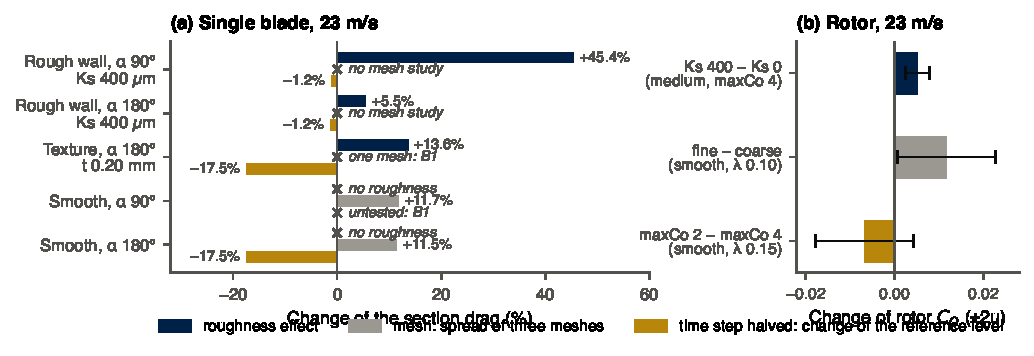
\includegraphics[width=\linewidth]{fig1_numerics}
\caption{Each roughness effect (navy) next to its family's change with the mesh (grey) and with a halved time
step (gold: maxCo 5 to 2.5 for the rough-wall and textured blades, 2.5 to 1.25 smooth, 4 to 2 rotor).
×: no such run.}
\label{fig:numerics}
\end{figure}

\textbf{B1} repeats each comparison at a smaller step and on other meshes (Table~\ref{tab:b1}). The texture setting stays if the smooth Cd(180) moves by at most \nAccLevel\,\% and the
drag rise stays within \nAccEff\ points of +\nTexEffLong\,\% with the same lift sign and shedding;
otherwise the finer setting is adopted (B2's texture runs then cost \nAccCostLo--\nAccCostHi\ times more).
The rotor gain stands if it is resolved on the fine mesh and at maxCo~2 and lies within \nAccRot\ of
\nRotEffTen; otherwise it is reported as mesh-dependent and no more rotor roughness runs are made.

\begin{table}[tbp]
\centering\footnotesize
\caption{The B1 runs (submitted 15 November) and the rough-wall mesh study (S2h, added the same day);
``now'': before B1. Results fill in as the runs finish (\nBoneDone\ of \nBoneQueueJobs\ B1 runs so far);
changes in \%, coarse/medium/fine in that order, rotor in C\textsubscript{Q}.}\label{tab:b1}
\begin{tabularx}{\linewidth}{@{}L{0.3} X L{0.36}@{}}
\toprule
Check (now) & Runs & B1 result \\
\midrule
T1 texture, α 180 (rise +\nTexEffLong) & maxCo 1.25, t 0 and 0.20~mm & level \nBoneTOneLevel; rise
\nBoneTOneEff \\
T2a texture, α 180, finer wall & 20\um\ spacing, maxCo 2.5 & level \nBoneTTwoLevel; rise \nBoneTTwoEff \\
E90 texture, edge-on (never run) & maxCo 2.5 and 1.25 & rise \nBoneTexNinetyA, \nBoneTexNinetyB \\
S1 smooth, α 180 (Cd \nMedCdTwoFive, \nMedCdOneTwoFive) & maxCo 0.625; coarse, fine at 1.25 & step
\nBoneSOneStep; meshes \nBoneSOneSpread \\
E90 smooth, edge-on (lift spread \nSpreadClNinety) & three meshes at maxCo 1.25 & Cd \nBoneNinetyCd; Cl
\nBoneNinetyCl \\
S2 smooth, α 0 (Cd \nZeroCdFive\ or \nZeroCdTwoFive) & 0.625; coarse, fine at 1.25; to 300 c/U; two
restarts & Cd \nBoneSTwoMed, \nBoneSTwoCoarse, \nBoneSTwoFine; restarts \nRestartContCd,
\nRestartHystCd \\
S2h rough wall, Ks 400 (no mesh study) & coarse and fine meshes, α 90 and 180 & rise α 90:
\nWfMeshNinetyCdC, \nWfMeshNinetyCdM, \nWfMeshNinetyCdF; α 180: \nWfMeshOneEightyCdC, \nWfMeshOneEightyCdM,
\nWfMeshOneEightyCdF \\
R1 rotor, λ 0.10 (\nRotEffTen\pmu\nRotEffTenU) & Ks 0, 400\um: fine; medium at maxCo 2; coarse &
\nBoneROneFine, \nBoneROneMedTwo, \nBoneROneCoarse; 2u \pending \\
\bottomrule
\end{tabularx}
\end{table}


\section{J2: how turbulence and roughness are modelled}\label{sec:j2}
All runs are 2D unsteady RANS (OpenFOAM v2606), mostly at 23~m/s, Tu~1\,\% and a 1~mm length scale
(Table~\ref{tab:families}; every setting: \nolinkurl{cfd/docs/SETUP_REVIEW_2026-11.md}).

\begin{table}[tbp]
\centering\footnotesize
\caption{The model families of the \nRunsAll\ October runs. SST: k-ω SST, fully turbulent. LM: k-ω SST with
γ--Re\textsubscript{θt} transition. Cells in thousands.}\label{tab:families}
\begin{tabularx}{\linewidth}{@{}L{0.2} L{0.17} X L{0.3}@{}}
\toprule
Family (runs) & Model (runs) & Wall; cells & How roughness enters \\
\midrule
Smooth blade (\nRunsSec) & SST (\nRunsSecSST), LM (\nRunsSecLM) & Resolved, y\textsuperscript{+} $<$ 1;
\nCellsSecLo--\nCellsSecHi & Not at all \\
Rough-wall blade (\nRunsWf) & SST & Wall function, y\textsuperscript{+} \nYplusWfLo--\nYplusWfHi;
\nCellsWf & Sand-grain Ks 0--400\um\ (Ks/y\textsubscript{P} $\le$ \nKsOverYpMax) \\
Textured blade (\nRunsTex) & SST (\nRunsTexSST), LM (\nRunsTexLM) & Resolved; \nCellsTex & Slicer's nominal
texture in the wall: ±t every 0.2~mm, one random pattern, 2D ridges \\
Rotor, 3 blades (\nRunsRotor) & SST & Wall functions; \nCellsRotLo--\nCellsRotHi; rotating & Ks 0, 100 or
400\um \\
\bottomrule
\end{tabularx}
\end{table}

\textbf{What none of the families represents.}
(1)~\emph{Transition triggered by roughness.} OpenFOAM v2606 has no such model. LM predicts transition from
free-stream turbulence and pressure gradient, not roughness, and the rough wall function assumes a
turbulent layer. Only the textured LM runs could show tripping, outside LM's calibration.
(2)~\emph{Our surface.} Ks was never measured (it needs a drag test, not a scan). The textured mesh uses the
slicer's nominal displacement. The G-code of the printed sets carries the same programmed texture (Ra
\nGcRaForty\ and \nGcRaEighty\um\ for FS~0.10 and 0.20, \nGcRatioLo--\nGcRatioHi\,t, as the synthetic
one), but filtered along the span like the scans it would read \nGcOverScanForty\ and
\nGcOverScanEighty\ times the measured Ra: the printed blades carry only part of it (smoothed by the
extruded bead, or missed by the scans; inferred). In 2D the texture also becomes ridges along the span,
expected to trip a layer more easily than the print's random 3D texture.
(3)~\emph{The tunnel and rig}: Tu and length scale are assumed; there are no tunnel walls, arms, hub or
blade tips, and the assembly is inferred from CAD.
The families also disagree on the smooth blade (α~180, maxCo~2.5: Cd \nCdWfSmooth, \nMedCdTwoFive\ and
\nTexCdSmooth\ on the rough-wall, smooth-blade and texture meshes), so this report compares only within a
family.

\section{J3: the flow around the blade and through the turn}\label{sec:j3}
On 15 November the wall pressure and friction of \nSurfCases\ single-blade runs (Fig.~\ref{fig:surface})
and each blade's torque, drag and lift through the turn in \nPfRuns\ rotor runs (Fig.~\ref{fig:phase}) were
extracted (\texttt{cfd/analysis/2026-11-15/}); all of it carries the uncertainty of Section~\ref{sec:j1}.

\textbf{Edge-on, rough wall} \indic. Ks~400\um\ moves the convex-side separation \nSSepShiftNinety\,c
upstream and weakens the convex side's suction peak (Cp \nSCpWfNinetyZero\ to \nSCpWfNinetyFour); the
convex face's pressure drag rises from \nSCdpWfNinetyZero\ to \nSCdpWfNinetyFour.

\textbf{Convex side to the wind, texture} \indic. At maxCo~2.5 the texture weakens the suction peak on the
tip-B side (Cp \nSCpTexZeroTwoFive\ to \nSCpTexTwoTwoFive) and moves separation \nSSepShiftTex\,c upstream.
At maxCo~5 the smooth run already has a weak peak (\nSCpTexZeroFive); the texture changes neither the peak
(\nSCpTexTwoFive) nor the separation, yet the drag rise is similar (+\nTexEffFive\,\%). Halving the time
step does the same to the smooth blade (peak \nSCpMedTwoFive\ to \nSCpMedOneTwoFive, separation
\nSSepShiftMed\,c upstream). The texture's drag rise is not yet tied to a mechanism.

\textbf{Through the turn, rotor} \indic. The Ks-400 gain comes from the advancing blade (θ~60--120°,
moving downwind edge-on): its drag about the relative wind rises by \nPfAdvCD\pmu\nPfAdvCDU\
(\nPfAdvCDPct\,\%) and there points along its path, so it drives; its lift changes more
(\nPfAdvCL\pmu\nPfAdvCLU) but acts along the arm. The returning blade's drag rises
(\nPfRetCD\pmu\nPfRetCDU) and brakes. Torque by sector: advancing \nSecAdv\pmu\nSecAdvU, returning
\nSecRet\pmu\nSecRetU, downwind \nSecDown\pmu\nSecDownU, upwind \nSecUp\pmu\nSecUpU. The blades differ by
more than 2u in \nPfBladeShare\,\% of the azimuth bins (\nPfBladeExpect\,\% expected), so these intervals
may be too narrow.

\textbf{Edge-on, texture} \indic. B1 ran the texture at α~90 for the first time: t~0.20~mm raises the drag
by \nBoneTexNinetyA\,\% at maxCo~2.5 and \nBoneTexNinetyB\,\% at 1.25, the blade position where the
rotor's gain sits, but on the 40\um\ wall that failed at α~180. Missing: its wall data and a 20\um\
check (B2), and surfaces on a turning blade (B2).

\begin{figure}[tbp]
\centering
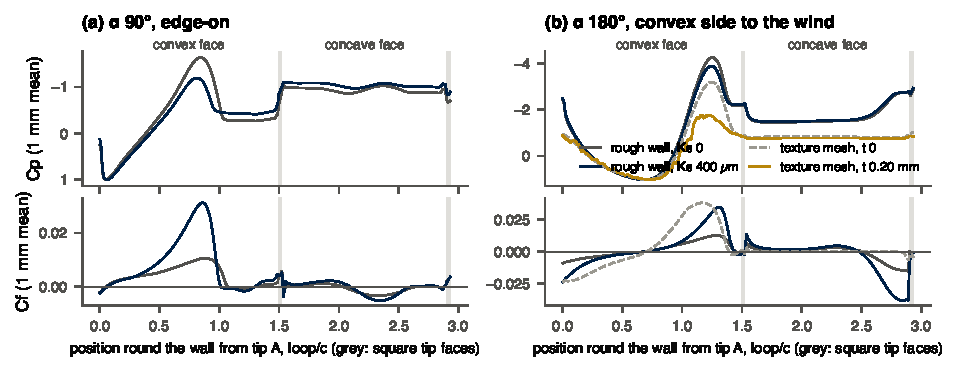
\includegraphics[width=\linewidth]{fig2_surface}
\caption{Time-mean wall pressure and friction round the blade (1-mm means; 23~m/s, SST, maxCo~2.5)
\nSurfFigState. (a) Edge-on. (b) Convex side to the wind; the textured wall's friction is omitted (it
reverses in the texture's valleys).}
\label{fig:surface}
\end{figure}

\begin{figure}[tbp]
\centering
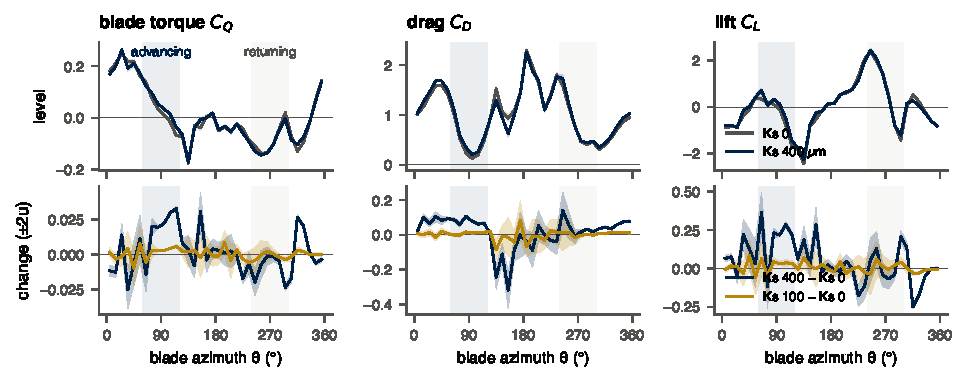
\includegraphics[width=\linewidth]{fig3_rotor_phase}
\caption{One blade's torque, drag and lift (about the relative wind) against azimuth: three-blade mean,
10° bins, λ~0.10, 23~m/s. Top: Ks~0 and 400\um; bottom: changes from Ks~0, ±2u. Shaded: advancing and
returning sectors.}
\label{fig:phase}
\end{figure}

\section{J4: why the gain appears only at high roughness}\label{sec:j4}
The CFD describes roughness by a sand-grain height Ks, never measured for a printed skin; three mappings give
different answers (Table~\ref{tab:mapping}).

\begin{table}[tbp]
\centering\footnotesize
\caption{Three mappings of the printed surfaces to Ks; \Ksp: blade mean of the runs at the nearest Ks.}\label{tab:mapping}
\begin{tabularx}{\linewidth}{@{}X L{0.2} L{0.12} L{0.2} L{0.11}@{}}
\toprule
Mapping & Plain, FS 0.05, FS 0.10 & FS 0.20 & \Ksp & Nearest case \\
\midrule
Ks = scanned height k (half the 1--99\,\% range) & \nKLow\um & \nKHighLo--\nKHighHi\um & section
\nKspSecLo--\nKspSecHi, rotor \nKspRotLo--\nKspRotHi & Ks 50--100\um \\
Measured Ra through the texture model (t = Ra/\nRaPerT, Ks = \nKsPerT\,t) & \multicolumn{2}{l}{all four:
\nKsEqLo--\nKsEqHi\um} & similar & Ks 50\um \\
Nominal slicer texture (Ks = \nKsPerT\,t) & 0, \nKsNomFsFive, \nKsNomFsTen\um & \nKsNomFsTwenty\um &
at 400\um: section \nKspSecFourLo--\nKspSecFourHi, rotor \nKspRotFour & Ks 200, 400\um \\
\bottomrule
\end{tabularx}
\end{table}

\textbf{From the scans} the blades sit at \Ksp\ \nKspSecLo--\nKspSecHi. The rough wall function is smooth
below \Ksp~\nKspSmoothLimit\ and transitional to \nKspRoughLimit, so it changes little there: at Ks 50 and
100\um\ the drag changes by \nWfNinetyFifty\ and \nWfNinetyHundred\,\% edge-on, \nWfOneEightyFifty\ and
\nWfOneEightyHundred\,\% at α~180 (Fig.~\ref{fig:ksplus}a). On the rotor the net change at Ks~100\um\ is
within its noise (\nRotHunTen\pmu\nRotHunTenU\ at λ~0.10, \nRotHunTwelve\pmu\nRotHunTwelveU\ at 0.12), but
the advancing sector's is resolved: \nAdvHun\pmu\nAdvHunU\ at λ~0.10, with the sign and place of the Ks-400
gain (Fig.~\ref{fig:ksplus}b). If the rotor's intervals are too narrow, as the blade-to-blade check in
Section~\ref{sec:j3} suggests, it is only marginally resolved. Growing linearly with Ks (assumed), the change would be \nTrendLo--\nTrendHi\
at \nKLow--\nKHighHi\um, below the 2u of \nRotTwoULo--\nRotTwoUHi\ from \nRevNow\ revolutions; resolving
it at \nKHighHi\um\ would take about \nRevNeeded\ revolutions per run.

\textbf{From the nominal texture}, FS~0.20 is the 400\um\ case, where the rotor gained \nRotEffTenPct\ and
\nRotEffTwelvePct\,\% (λ~0.10, 0.12). So ``gains only at high roughness'' may read ``gains at the Ks the
nominal texture implies, unresolved at the Ks the scans imply''. Only this mapping orders the sets as the
gains do (FS~0.10: \nGainFsTen\,\% [\nGainFsTenLo, \nGainFsTenHi]; the scans give it the same or a lower Ks
than Plain), but its Ra is \nNomOverRaLo--\nNomOverRaHi\ times the measured one. B2's Ks sweeps (rotor 25,
50, 200\um; section 25--211\um) will give each FS an equivalent Ks: \pending. \Ksp\ describes a turbulent
rough wall; tripping a laminar layer is a separate question that no family represents.

\begin{figure}[tbp]
\centering
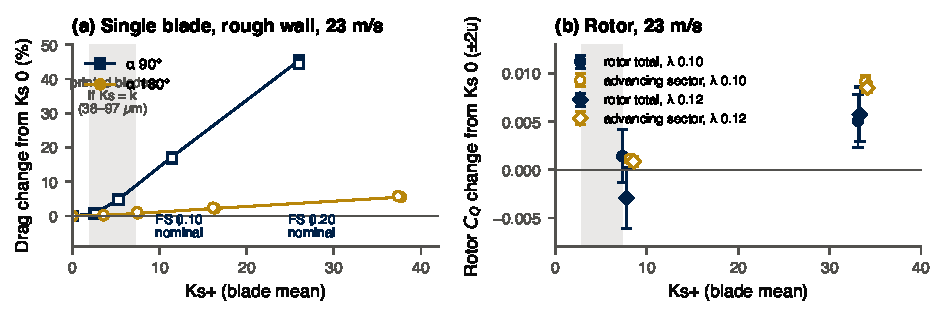
\includegraphics[width=\linewidth]{fig4_ksplus}
\caption{Roughness effect against \Ksp: (a) single-blade drag, rough wall (filled: maxCo~2.5; open: 5;
ticks: nominal Ks of FS~0.10, 0.20); (b) rotor torque, all blades and advancing sector (±2u). Grey: the
printed blades if Ks equals the scanned height.}
\label{fig:ksplus}
\end{figure}

\section{The tunnel and the blades}\label{sec:tunnel}
\textbf{Blades.} Each tested level has one print, and Plain was printed with thicker layers than the
textured sets (Table~\ref{tab:blades}). On measured Ra all four tested sets look like a nominal t of \nTeqLo--\nTeqHi~mm,
nearest the new FS~0.025 set; Plain is the roughest.

\begin{table}[tbp]
\centering\footnotesize
\caption{Blade sets and their CFD stand-ins (t: fuzzy-skin thickness; layer from the scans unless marked;
G-code: \texttt{blades/as\_printed/}).}\label{tab:blades}
\begin{tabularx}{\linewidth}{@{}L{0.14} L{0.12} X L{0.08} L{0.15} L{0.15}@{}}
\toprule
Set (t, mm) & Nozzle; layer (mm) & G-code & Ra (µm) & Stand-in, nominal & Stand-in, measured \\
\midrule
Plain (0) & \nNozzleSmall$^{a}$; \nLayerPlain & no slicer record & \nRaPlain & t 0 & t \nTeqPlain; k
\nKLow\um \\
FS 0.05 (\nTFsFive) & \nNozzleSmall; \nLayerFsFive & ``Ra20'' file has no fuzzy skin; source unconfirmed
& \nRaFsFive & t 0.05 (maxCo 5); Ks \nKsNomFsFive\um & t \nTeqFsFive; k \nKLow\um \\
FS 0.10 (\nTFsTen) & \nNozzleSmall; \nLayerFsTen & ``Ra40'' (plate 40~RA) & \nRaFsTen & t 0.10; Ks
\nKsNomFsTen\um & t \nTeqFsTen; k \nKLow\um \\
FS 0.20 (\nTFsTwenty) & \nNozzleSmall; \nLayerSlicer\ (slicer) & ``Ra80'' (plate 80~RA) & \nRaFsTwenty & t
0.20; Ks \nKsNomFsTwenty\um & t \nTeqFsTwenty; k \nKHighLo--\nKHighHi\um \\
\addlinespace
Sets 1--3: Plain, FS 0.40, FS 0.025 (\nTFsQuarter) & Plain \nNozzleLarge; others to confirm & due about
23 Nov; ``10 RA'' G-code exists & --- & t 0; no mesh (Ks \nKsNomFsForty\um); t 0.025 (Ks
\nKsNomFsQuarter\um) & after scans \\
FS 0.805 (\nTFsEighty) & \nNozzleLarge; \nLayerFsEighty\ (slicer) & ``320 RA'', sliced only & --- & no mesh & --- \\
\bottomrule
\end{tabularx}
\par\smallskip\raggedright $^{a}$Stated by the Print Lab, but Plain's \nLayerPlain-mm layers exceed the
\nLayerLimit-mm limit of its \nNozzleSmall-mm profile.
\end{table}

\textbf{Rotor speed through the loading (J7)} was logged at all \nDwells\ load steps of the tested sets
(\nDwellsOk\ valid). At 23~m/s the tip-speed ratio falls from \nLamLightLo--\nLamLightHi\ at the lightest
load to \nLamHeavyLo--\nLamHeavyHi\ at the heaviest, through the CFD's λ~0.10 and 0.12; peak power is at
\nLamPmaxLo--\nLamPmaxHi\ (Fig.~\ref{fig:speed}). The new sets need the same record.

\begin{figure}[tbp]
\centering
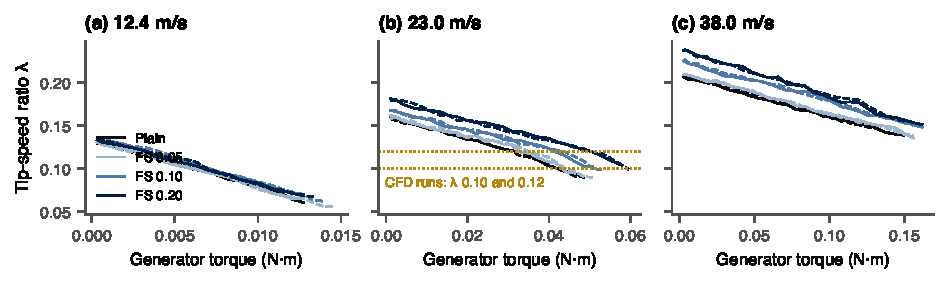
\includegraphics[width=\linewidth]{fig5_rotor_speed}
\caption{Tip-speed ratio against generator torque (electromagnetic, without bearing friction) through each
load sweep of 1 October; solid: run~1, dashed: run~2.}
\label{fig:speed}
\end{figure}

\textbf{Blade forces (J5)}, to decide with R.\ Cassin and Y.\ Kim by about 24 November:
(1)~\emph{build the docs/12 balance} (two load cells under the floor, a blade half in the wind; parts \$\nBalLentLo--\nBalLentHi\ if the lab lends the pitot tube, manometer and plate
stock, \$\nBalLo--\nBalHi\ otherwise; on hold); (2)~\emph{borrow a balance} from another lab (the MCE lab
has none to lend, 4 November);
(3)~\emph{static torque}, the rotor held at set angles (simpler, but rotor torque only, not blade lift and
drag); (4)~\emph{pressure taps} on a printed section (cheap; Cp for J3, but no viscous drag, which is up to
\nPressViscMax\,\% of Cd in the \nHealthyRuns\ healthy smooth-blade runs).

\textbf{Replicates and cost.} Second prints on one nozzle and layer height, with a matched Plain, would
separate texture from print and mounting effects. Print Lab estimates per blade
(\$\nPrintRate\ per print hour plus filament at \$\nFilament/kg, its 12 October rate, assumed here): Plain on
the \nNozzleLarge-mm nozzle \nPrintPlainFourH~h, \nPrintPlainFourG~g, \$\nPrintPlainFourUsd; FS~0.40
\nPrintFsFortyH~h, \nPrintFsFortyG~g, \$\nPrintFsFortyUsd; FS~0.025 \nPrintFsQuarterH~h, \nPrintFsQuarterG~g,
\$\nPrintFsQuarterUsd. The new sets and J5--J7 need about \nTunnelLo--\nTunnelHi\ tunnel hours, from about
18 December.

\section{Computing and the decisions needed}\label{sec:computing}
The October runs used about \nOctCoreH\ core-hours in \nOctJobs\ Unity jobs (28 October summary); the job
records on the Mac cover \nLocalJobs\ jobs and \nLocalCoreH\ core-hours. Unity now rejects any job that
asks for more than \nUnityDays\ days; the longest B1 job is estimated at \nBoneLongestDays\ days
(plan: Table~\ref{tab:compute}). COMSOL on Unity is licensed to UMass Amherst and would not remove the cost
of resolving the texture; we do not plan to use it.

\begin{table}[tbp]
\centering\footnotesize
\caption{Computing planned (estimates; B1 from its queue files, the rest from the plan of 15 November).}\label{tab:compute}
\begin{tabularx}{\linewidth}{@{}L{0.28} L{0.33} X@{}}
\toprule
Item & Core-hours & Status \\
\midrule
B1 verification, \nBoneJobs\ jobs & \nBoneCoreLo--\nBoneCoreHi & Submitted 15 Nov \\
B2 mechanisms (SST) & \nBTwoLo--\nBTwoHi & After B1 is read \\
Textured 2D rotor & \nTexRotRevLo--\nTexRotRevHi\ per revolution (now \nCoreHPerRev); 15-revolution pair
\nTexRotPairLo--\nTexRotPairHi & After B1 and B2 \\
LM rotor (transition) & \nLmRotLo--\nLmRotHi & After B1 and B2 \\
3D strip, 1--2~mm of span & \nStripLo--\nStripHi\ per case & Exploratory \\
Full 3D blade, \nBladeCellsLo--\nBladeCellsHi\ billion cells & \nBladeCoreLo--\nBladeCoreHi\ million per
case (\nBladeOverOctLo--\nBladeOverOctHi\ × October) & Not feasible \\
\bottomrule
\end{tabularx}
\end{table}

\textbf{Decisions needed.} (1)~The force test (J5), about 24 November. (2)~B2: go or no-go, with R.\ Cassin, after
reading B1 (about 23--25 November); by the B1 rules its texture runs move to the 20\um\ wall (cost
\nAccCostLo--\nAccCostHi\ times). (3)~A smaller-step check of the wall-resolved smooth blade (maxCo about
0.3 at α~90 and 180), which B1 showed is not converged. (4)~Second prints on one nozzle and layer height, with a matched Plain. (5)~A speed record for the new
sets (J7). (6)~The textured or LM rotor, a mesher for FS~0.40 and 0.805, or the 3D strip: after B2.

\section{Corrections to the 28 October summary}\label{sec:corrections}
(1)~It said the single-blade runs varied ``the printed texture shape itself''. The \nRunsTex\ texture runs
use a synthetic stand-in: the slicer's nominal displacement as 2D ridges, with an Ra
\nNomOverRaLo--\nNomOverRaHi\ times the measured one. The printed sets' G-code has the same programmed
texture, so the stand-in matches what was programmed, not what was printed (Section~\ref{sec:j2}).
(2)~It said the 100\um\ cases ``are the closest to the real blades''. That holds only if Ks equals the
scanned height; with the nominal texture, FS~0.10 and FS~0.20 correspond to about \nKsNomFsTen\ and
\nKsNomFsTwenty\um, the latter the 400\um\ case that gained (Section~\ref{sec:j4}).
(3)~It gave the balance parts as \$\nBalOldLo--\nBalOldHi; the design gives \$\nBalLentLo--\nBalLentHi\ with
borrowed parts, \$\nBalLo--\nBalHi\ without.

{\tiny\color{ink2}\textbf{Provenance.} Built \BuildDate, git \BuildGit, by \texttt{make\_figures.py}
(every number, with its source, in \texttt{numbers.tex}). Inputs and SHA-256 prefixes (tracked in git unless
marked local, git-ignored and on the analysis Mac only, or untracked, not yet committed): \ProvenanceList\par}

\end{document}
